\documentclass[a4paper,12pt]{article}

\usepackage{amsmath,amssymb,multicol,tikz,enumitem}
\usepackage[margin=2cm]{geometry}
%\usetikzlibrary{calc}
\usepackage{amsmath}
\usepackage{amsthm}
\usepackage{thmtools}
\usepackage{hyperref}
\usepackage{enumerate}
\usepackage{xcolor}

\pagestyle{empty}

\newcommand\Q{\mathbf{Q}}
\newcommand\R{\mathbf{R}}
\newcommand\Z{\mathbf{Z}}

\newcommand\answer[1]{}
\newcommand\ans[1]{}
%\newcommand\answer[1]{\\[5pt]{\color{blue}{#1}}\hfill{\color{blue}}\\[-5pt]}
%\newcommand\ans[1]{{\color{blue}{#1}}}

\usepackage{array}
\newcolumntype{P}[1]{>{\centering\arraybackslash}p{#1}}

\newcommand\indd{${}$\hspace{20pt}}

\declaretheoremstyle[headfont=\normalfont\bfseries,notefont=\mdseries\bfseries,bodyfont = \normalfont,headpunct={:}]{normalhead}
\declaretheorem[name={Uzdevums}, style=normalhead,numberwithin=section]{problem}

\setcounter{section}{01}

\setlength\parindent{0pt}

\renewcommand{\figurename}{Attēls}

\begin{document}

\begin{center}
\parbox{3.5cm}{\flushleft\bf Decimālpieraksts} \hfill {\bf\LARGE Sacensības \#2021.03} \hfill \parbox{3.5cm}{\flushright\bf 2021-25-03} \\[2pt]
{\rm\footnotesize Par šo LU NMS atbalstīto pasākumu\\ atbild {\tt kalvis.apsitis@gmail.com}.}
\end{center}

%\hrule\vspace{2pt}\hrule
\hrule

%\vspace{10pt}
%{\bf Iesniegšanas termiņš:} 2021.g.\ 20.februāris\\
%{\bf Kam iesūtīt:} {\tt kalvis.apsitis}, domēns {\tt gmail.com}

%{\large\bf Eratostēna režģis.}

%\vspace{10pt}
%\begin{figure}[!htb]
%\center{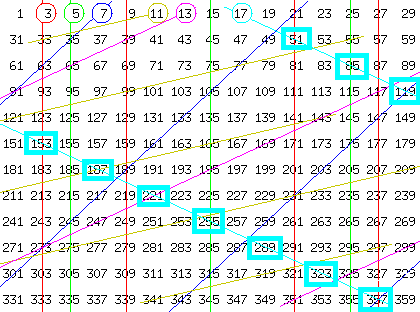
\includegraphics[width=3in]{online-competition-2021-02-18/eratosthenes-with-17.png}}
%\caption{\label{fig:eratosthenes-with-17} Eratostēna režģis nepāru skaitļiem.}
%\end{figure}

\vspace{10pt}
\begin{problem}
Ar $n$ apzīmēts mazākais naturālais skaitlis, kas dalās ar $56$ un kura de\-ci\-māl\-pie\-rak\-stā ir tikai cipari $0$ vai $3$. Atrast šo $n$.

{\bf Jautājums:} Ierakstīt atbildē naturālu skaitli.
\answer{

{\bf Atbilde.} $\mathtt{3003000}$

Tā kā $56=7 \cdot 2^3$, tad ir nepieciešami un pietiekami, lai skaitlis dalītos
ar abām pirmreizinātāju pakāpēm (t.i.\ gan ar $7$, gan ar $8$). 

Lai skaitlis, kura beigās ir nepāru cipars ($3$), dalītos ar $8$, tam galā jāpieraksta trīs nulles.
Savukārt, mazākais skaitlis, kas dalās ar $7$ (no cipariem $3$ un $0$) ir $3003$.
To pārbaudām, izmēģinot dalīt $3$, $33$, $303$, $333$ ar $7$ (un pārliecināties, ka tie nedalās).\\
Tāpēc dalāmībai ar $7$ jāizvēlas nākamais mazākais skaitlis $3003$.

Tātad rezultāts ir $3003 \cdot 1000 = 3003000$.
}
\end{problem}

\vspace{10pt}
\begin{problem}
Sakārtotu pāri $(k,m)$ ar nenegatīviem veseliem skaitļiem sauksim par vienkāršu,
ja, saskaitot $k$ un $m$ stabiņā, nerodas pārnesumi.
Atrast, cik ir vienkāršu pāru $(k,m)$, kuriem summa $k+m=1492$.

{\bf Jautājums:} Ierakstīt atbildē naturālu skaitli \textendash{} sakārtotu pāru kopskaitu ar aprakstīto īpašību.
\answer{

{\bf Atbilde.} $\mathtt{300}$\\
\textcolor{teal}{\bf Daļēja Atbilde.} $\mathtt{298}$

Pavisam sakārtotu pāru ar vajadzīgo summu ir $1492+1 = 1493$. Sākot ar $(0;1492)$, $(1;1491)$, $\ldots$, $(1492;0)$.

No tiem daži ir tādi, kuros nav pārnesumu.\\
Tūkstošu ciparā var būt $0+1$ vai $1+0$ (pavisam divi veidi iegūt summā $1$).\\
Simtu ciparā var būt $0+4 =1+3=2+2=3+1=4+0$ (pavisam pieci veidi kā iegūt $4$).

Veidu skaits katrā decimālpieraksta pozīcijā ir par vienu lielāks nekā attiecīgais cipars.
Tādēļ veidu skaitu varam izteikt kā reizinājumu:
\[ (1+1) \cdot (4+1) \cdot (9+1) \cdot (2+1) = 300. \]

{\em Piezīme.} Pārnesumu skaits dažreiz ir svarīgs arī uzdevumos, kas nav saistīti ar skaitļa pierakstu
\textendash{} sk.\ {\em Kummera teorēmu} (\url{https://bit.ly/2QFwrb9}), kas ļauj pareģot, 
ar kādu pirmskaitļa $p$ pakāpi dalīsies kombināciju skaits $C_n^k$. Bet šajā uzdevumā tas
nedarbojas, jo $10$ nav pirmskaitlis.

Ja skaita nevis pārus ar veseliem nenegatīviem skaitļiem, bet ar naturāliem skaitļiem (t.i.\ neatļauj 
pārus $(0;1492)$ un $(1492;0$), tad sanāk atbilde $298$, kas skaitās daļēji pareiza.
}
\end{problem}


\vspace{10pt}
\begin{problem}
Katram naturālam skaitlim $n$ apzīmējam ar $f(n)$ tā ciparu kvadrātu summu.\\
Atrast vērtību $f^{2021}(123456789)$, kur $f^2(n)=f(f(n))$, $f^3(n)=f(f(f(n)))$; un $f^{2021}(n)$ apzīmē funkcijas pielietošanu $2021$ reizi.

{\bf Jautājums:} Ierakstīt atbildē naturālu skaitli, $f^{2021}(123456789)$ vērtību.
\answer{

{\bf Atbilde.} $\mathtt{4}$\\
\textcolor{teal}{\bf Daļēja Atbilde.} $\mathtt{20}$ (neliela nobīde pa ciklu)

Skaitļa ciparu kvadrātu summa (atšķirībā no parastās ciparu summas, kas kalpo 
kā pazīme dalāmībai ar $3$ un ar $9$) nav pazīstama kā
svarīga pazīme vai invariants.

Toties viegli pamatot, ka pēc kāda laika ciparu kvadrātu summa ieciklosies
(lielām $n$ vērtībām virkne $n, f(n), f(f(n)),\ldots$ vispirms strauji dilst, 
bet pēc tam nonāk intervālā $[1;199]$, no kura ārā vairs nekad netiek, jo $1^2 + 9^2 + 9^2 \leq 199$).
Tāpēc neizbēgami kaut kad šajā virknē parādīsies divas vienādas vērtības $f^k(n)$ un 
$f^m(n)$, kam $k \neq m$. 

Mūsu gadījumā ``satikšanās punkts'' ir  $f^7(123456789)=f^{15}(123456789)$, 
t.i. iegūstam virkni ar priekšperioda garumu $7$ un perioda garumu $8$. 

\begin{figure}[!htb]
\center{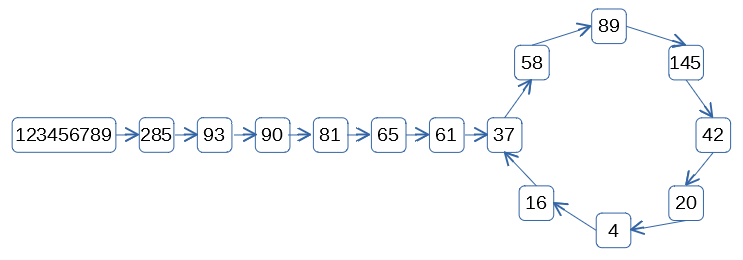
\includegraphics[width=5in]{online-competition-2021-03-25/q3-periodic.png}}
\caption{\label{fig:q3-periodic} Ciparu kvadrātu summu virkne ar priekšperiodu un periodu.}
\end{figure}

Kāds ir šīs virknes 2021.loceklis? Atņemam priekšperiodu un dalām ar periodu: 
$(2021 - 7)$ dod atlikumu $6$, dalot ar $8$. Tāpēc $f^{2021}(123456789) = 4$, kas ir 6.skaitlis
periodā (sk. astoņstūraino ciklu Attēlā~\ref{fig:q3-periodic}).

{\em Piezīme.} Priekšperiods šajā situācijā rodas tādēļ, ka $f(16) = f(61) = 37$, t.i.\ diviem 
atšķirīgiem $n_1 = 16$ un $n_2 = 61$ funkcijas vērtības sakrīt: $f(n_1) = f(n_2)$. 
Šādu situāciju sauc par ``kolīziju'' jeb ``sadursmi'' un tad arī saka, ka funkcija $f$ nav injektīva, 
jo skaitlim $37$ eksistē divi dažādi skaitļi ($16$ un $61$), kuri par to attēlojas. 
(Sk.\ \url{https://bit.ly/3spwxlc}).
}
\end{problem}


\vspace{10pt}
\begin{problem}
Pieņemsim, ka $n$ ir naturāls skaitlis un $d$ ir cipars (no $0$ līdz $9$). Atrast $n$, ja zināms, ka
\[ \frac{n}{810}=0.d25d25d25... = 0.(d25) \]
ir bezgalīga periodiska daļa.

{\bf Jautājums:} Ierakstīt atbildē naturālu skaitli $n$.
\answer{

{\bf Atbilde.} $\mathtt{750}$\\
Šo uzdevumu var efektīvi risināt ar ``pilno pārlasi: Var reizināt visus skaitļus $0.(025)$, $0.(125)$, $\ldots$, $0.(925)$
ar $810$, kamēr iegūstam veselu skaitli (jāpārbauda tikai $10$ iespējas). 

Bet tā kā olimpiādēs kalkulatorus parasti nevar izmantot, 
papūlēsimies atrast analītisku risinājumu. 
Ievērojam, ka $1/999 = 0.(001)$, tāpēc katrs skaitlis ar 3-ciparu periodu ir pierakstāms kā $\overline{d25}/999$. Tā kā $999$ dalās ar $37$, 
bet $810$ nedalās ar $37$, tad ar $37$ jāvar noīsināt daļā $\overline{d25}/999$. Vienīgais skaitlis, kurš dalās ar $37$ būs $925 = 37 \cdot 25$, 
tātad cipars $d=9$.

Visbeidzot atrisinām $\frac{925}{999} = \frac{n}{810}$. Iegūstam $n = 750$.
}
\end{problem}


\vspace{10pt}
\begin{problem}
Apzīmēsim ar $A$ racionālo skaitļu apakškopu. Racionāls skaitlis $r \in A$ tad un tikai tad, ja $0<r<1$ un
\[ r=0.abcabcabc...=0.(abc) \]
tātad $r$ izsakāms kā bezgalīga decimāldaļa ar periodu $3$ cipari ($a,b,c$ - starp tiem var būt arī vienādi cipari), bet bez priekšperioda.

Ja visus kopas $A$ elementus uzraksta kā nesaīsināmas daļas, cik dažādi skaitītāji ir visām šīm daļām kas pieder $A$?

{\bf Jautājums:} Ierakstīt naturālu skaitli: dažādo skaitītāju skaitu, kas iespējami daļām $p/q=r$, kur $r \in A$.
\answer{

{\bf Atbilde.} $\mathtt{660}$\\
\textcolor{teal}{\bf Daļēja Atbilde.} $\mathtt{648}$

Tā kā $1/999 = 0.001001\ldots = 0.(001)$, tad visus $r \in A$ var uzrakstīt kā $n/999$, 
kur $n = 1,\ldots,998$ un daļa $n/999$, iespējams, ir saīsināma. 

Noskaidrosim, kurām $n$ vērtībām tā ir saīsināma. Sadalām pirmreizinātājos $999 = 3^3 \cdot 37$. 
Tāpēc $n$ vērtības, kuras dalās ar $3$ vai ar $37$ tūlīt varēs saīsināt. 
Tas gan nenozīmē, ka pēc saīsināšanas $n/999 = p/q$ nevar iegūt tādu daļas skaitītāju $p$, kas 
dalītos ar $3$. Jo izrādās, ka $999$ dalās ar $27$, bet ir arī $12$ tādi skaitļi ($81, 162, \ldots, 972$), 
kuri dalās ar $81$, un kuri izveido vēl divpadsmit tādas daļas $p/q$, kurām pirmreizinātāji 
$3^k$ noīsinās tikai daļēji (jo $999$ dalās ar $3^3$, bet ar augstākām $3$ pakāpēm tas nedalās). 

\begin{figure}[!htb]
\center{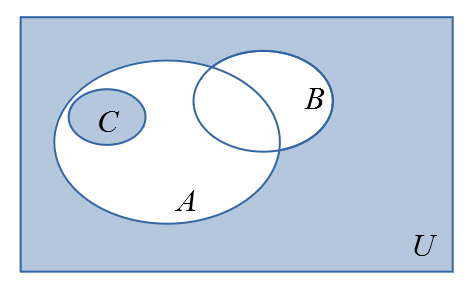
\includegraphics[width=2in]{online-competition-2021-03-25/q5-euler.png}}
\caption{\label{fig:q5-euler} Eilera diagramma skaitļu kopām, kas dalās ar $3$, ar $37$, ar $81$.}
\end{figure}

Lai šo situāciju uzskatāmāk saprastu, ieviesīsim šādas kopas:\\
Kopa $U$ satur visus $n \in [1;998]$ (vislielāko kopu, kurā veic visas darbības, sauc par ``universu''),\\
Kopa $A$ satur tos $n \in [1;998]$, kas dalās ar $3$,\\
Kopa $B$ satur tos $n \in [1;998]$, kas dalās ar $37$,\\
Kopa $C \subset A$ satur tos $n \in [1;998]$, kas dalās ar $81$,\\
Kopa $A \cup B$ satur tos $n \in [1;998]$, kas dalās ar $3$ vai ar $37$ (kopu $A$, $B$ apvienojums),\\
Kopa $A \cap B$ satur tos $n \in [1;998]$, kas dalās ar $3$ un ar $37$ (kopu $A$, $B$ šķēlums).

Attēlā~\ref{fig:q5-euler} attēlota Eilera diagramma (atšķirībā no Venna diagrammas, tai jāattēlo nevis visi $2^3 = 8$ 
reģioni, ko veido trīs šķeļo bet tikai tie, kuri reāli eksistē; tātad $C$ var zīmēt kopas $A$ iekšpusē.

Unikālus daļu skaitītājus dod tikai tie reģioni, kuri Attēlā~\ref{fig:q5-euler} iekrāsoti (t.i. vai nu 
atrodas ārpus $A$ un $B$, vai arī atrodas kopā $C$ un izveido daļas skaitītāju, kurš dalās ar $3$). 

Ja kopu elementu skaitu apzīmējam ar $|U|$, $|A|$, $|B|$, $|C|$, tad iegūsim šādu izteiksmi iekrāsotajam reģionam: 
\[ |U| - |A \cup B| + |C| = |U| - (|A| + |B| - |A \cap B|) + |C| = 998 - (332 + 26 - 8) + 12 = 660. \]
Mēs te izmantojām to, ka elementu skaits kopā $A$ ir $|A| = \lfloor 998/3 \rfloor = 332$,\\
$|B| = \lfloor 998/37 \rfloor = 26$,\\
$|A \cap B| = \lfloor 998/111 \rfloor = 8$,\\
$|C| = \lfloor 998/81 = 12 \rfloor$.

Sakarību, kas ļauj pārrakstīt $|A \cup B|$ par $|A| + |B| - |A \cap B|$ kombinatorikā sauc 
par ieslēgšanas-izslēgšanas principu; sk.\ \url{https://bit.ly/2P6ZqUM}.

{\em Piezīme.} Tie, kuri aizmirsa pieskaitīt $12$ (visus tos skaitļus, kuriem daļas $n/999$ skaitītājs dalās
ar $81$ un tāpēc nenoīsinās pilnībā ar $999$), ieguva atbildi $648$, ko uzskatām par daļēji pareizu.
}
\end{problem}


\vspace{10pt}
\begin{problem}
Katram naturālam skaitlim $n$ ar $p(n)$ apzīmējam visu nenulles ciparu rei\-zi\-nā\-ju\-mu skaitlī $n$.
(Ja skaitlī $n$ ir tikai viens cipars, tad $p(n)=n$.). Aprēķinām
\[ S = p(1)+p(2)+...+p(999). \]
Atrast skaitļa $S$ lielāko pirmreizinātāju.

{\bf Jautājums:} Ierakstīt atbildē lielāko pirmskaitli, ar kuru dalās $S$.
\answer{

{\bf Atbilde.} $\mathtt{103}$

Sasummējam pirmos $9$ skaitļus (apzīmējam to ar $S_1$:
\[ S_1 = 1 + 2 + \ldots + 9 = \frac{9 \cdot 10}{2} = 45. \]
Sasummējam arī līdz $p(99)$ (apzīmējam to ar $S_2$):
\begin{align}
S_2 = & (p(1) + p(2) + \ldots + p(9)) + (p(10) + p(11) + p(12) + \ldots p(19)) + \ldots + (p(90) + \ldots p(99)) = \nonumber \\
= & S_1 +  S_1 \cdot (1 + (1 + 2+\ldots 9)) = 45  + 45 \cdot 46 = 2115. \nonumber
\end{align}

Tālāk apskatām visus skaitļus no $1$ līdz $999$ (izņemot pilnos simtus $100$, $200$, $300$, $\ldots$, $900$) sagrupējam 
desmit grupās (atkarībā no simtu cipara):
\begin{align}
S_3 = &(p(1) + \ldots + p(99)) + (p(101) + \ldots + p(199)) + \ldots + (p(901) + \ldots + p(999)) = \nonumber \\
= & 1 \cdot S_2 + 1 \cdot S_2 + 2 \cdot S_2 + \ldots + 9 \cdot S_2 = \nonumber \\
= & (1 + 1 + 2 + \ldots + 9) \cdot S_2 = 46 \cdot 2115 = 97290.
\end{align}

Visbeidzot pieskaitām $p(100) + p(200) + \ldots + p(900) = S_1 = 45$. Iegūstam 
\[ S = 97290 + 45 = 97335. \]
Dalām pirmreizinātājos: 
\[ 97335 = 27 \cdot 3605 = 27 \cdot 5 \cdot 721 = 27 \cdot 5 \cdot 7 \cdot 103. \]
Lielākais pirmreizinātājs ir $103$.
}
\end{problem}

\vspace{10pt}
\begin{problem}
Atrast mazāko naturālo k ar īpašību, ka $16^k \equiv 1 \pmod{41}$.

{\bf Jautājums:} Ierakstīt atbildē mazāko naturālo kāpinātāju $k$,
kuram $16^k$ dod atlikumu $1$, dalot ar $41$.
\answer{

{\bf Atbilde.} $\mathtt{5}$

Kāpinot (pēc $41$ moduļa), varam atrast 
\[ \left\{ \begin{array}{l}
16^1 \equiv 16 \pmod{41},\\ 
16^2 \equiv 10 \pmod{41},\\ 
16^3 \equiv 37 \pmod{41},\\ 
16^4 \equiv 18 \pmod{41},\\
16^5 \equiv 1 \pmod{41}.\\
\end{array} \right.
\]
Tātad jau pie $k=5$ atlikums $16^k$, dalot ar $41$, būs $1$. Ievērojiet, ka tas notiek daudz ātrāk nekā 
tas, ko prognozē Mazā Fermā teorēma ($16^{40} \equiv 1 \pmod {41}$), jo pēc šīs teorēmas periods iestājas pēc $p-1 = 40$ soļiem, ja
pirmskaitlis $p = 41$.

{\em Piezīme.} Mazāko skaitli $k$, kuram $a^k \equiv 1 \pmod{p}$ sauc par skaitļa $a$ multiplikatīvo kārtu (pēc pirmskaitļa $p$ moduļa). 
Tātad skaitļa $16$ multiplikatīvā kārta ir $5$ $\pmod{41}$. Sk.\ \url{https://bit.ly/31gCpBe}. Viegli pamatot, ka multiplikatīvā 
kārta vienmēr ir skaitļa $p-1$ dalītājs, lai būtu ievērota M.Fermā teorēma.
}
\end{problem}


\vspace{10pt}
\begin{problem}
Heksadecimālajā sistēmā (ar bāzi $B=16$) lieto šādus ciparus:
\[ \mathtt{0},\mathtt{1},\mathtt{2},\mathtt{3},\mathtt{4},\mathtt{5},\mathtt{6},\mathtt{7},\mathtt{8},
\mathtt{9},\mathtt{A},\mathtt{B},\mathtt{C},\mathtt{D},\mathtt{E},\mathtt{F}. \]
Piemēram, cipara $\mathtt{F}_{16}$ vērtība ir $15$ (decimāli),
bet cipara $\mathtt{A}_{16}$ vērtība ir $10$ (decimāli).
Skaitlis $\mathtt{FFF}_{16}$ apzīmē $15 \cdot B^2 + 15 \cdot B + 15 = 15 \cdot 256+15 \cdot 16+15=4095$.

Heksadecimālajā sistēmā var pierakstīt arī daļskaitļus. Piemēram,
\[ \mathtt{0.AA}_{16} = 10 \cdot B^{-1} + 10 \cdot B^{-2}=10 \cdot \frac{1}{16} + 10 \cdot \frac{1}{16^2} = 0.6640625. \]
\[ \mathtt{0.0F0F0F...}_{16}=\mathtt{0.(0F)}_{16} = 15 \cdot \left( \frac{1}{256} \right) +15 \cdot \left( \frac{1}{256} \right)^2+ \ldots= \frac{1}{17}. \]
(Summēšanai izmanto bezgalīgu ģeometrisko progresiju.)

Atrast perioda ciparus skaitļa $1/41$ heksadecimālajā pierakstā (šeit skaitlis $41$ pierakstīts decimāli).

{\bf Jautājums:} Ierakstīt atbildē perioda ciparus skaitlim $1/41$ (bez nulles, punkta vai iekavām).
Teiksim, $1/17$ gadījumā atbilde būtu $\mathtt{0F}$.
\answer{

{\bf Atbilde.} $\mathtt{063E7}$

Iepriekšējā jautājumā jau noskaidrojām, ka $16^5 - 1 = 1048575$ dalās ar $41$; dalīšanas rezultāts ir 
$(16^5 - 1)/41 = 25575$. Tāpēc
\[ \frac{1}{41} = \frac{25575}{1048575} = 25575 \cdot \frac{1}{16^5 - 1} = 
25575 \cdot \left( \frac{1}{16^5} + \frac{1}{16^{10}} + \frac{1}{16^{15}} + \frac{1}{16^{20}} + \ldots \right). \]
Pēdējā vienādība seko no bezgalīgas ģeometriskas progresijas summas formulas.

Pārveidojam šo daļu heksadecimālajā skaitīšanas sistēmā:
\begin{equation}
\label{eq:infinite-hex}
\frac{1}{1048575} = 0.000010000100001\ldots_{16}.
\end{equation}
Pārveidojam $25575_{10}$ par heksadecimālu skaitli, atkārtoti dalot ar $16$:
\[
\begin{array}{l}
25575 = 1598 \cdot 16 + 7,\\
1598 = 99 \cdot 16 + 14,\\
99 = 6 \cdot 16 + 3,\\
6 = 0 \cdot 16 + 6.\\
\end{array}
\] 
Tāpēc $25575_{10} = \mathtt{063E7}_{16}$. Tagad reizinām to ar (\ref{eq:infinite-hex})
(jeb dalām ar $1048575$ lai iegūtu precīzi $\frac{1}{41}$). Iegūstam:
\[ \frac{25575}{1048575} = \frac{1}{41} = \mathtt{0.063E7063E7063E7...}_{16} = \mathtt{0.(063E7)}_{16}. \]

{\em Piezīme.} Šis pieraksts $\mathtt{0.063E7063E7}\ldots$ ir tieši tas, kā skaitlis $\frac{1}{41}$ glabājas datora atmiņā 
(jo tur arī daļskaitļus glabā bināri, nevis decimāli). 
Daļskaitļus un ``peldošā punkta'' skaitļus ({\tt float}, {\tt double} tipi daudzās programmēšanas valodās) noapaļo, 
lai tie ietilptu $4$-baitu vai $8$-baitu atmiņas reģistrā. Viens baits jeb astoņi biti ir divi heksadecimālie cipari, jo $16^2 = 2^8$.
}
\end{problem}


\vspace{10pt}
\begin{problem}
Skaitli $r$ var uzrakstīt kā decimāldaļu ar četriem cipariem aiz komata: $0.abcd$, kur $a,b,c,d$ ir jebkuri cipari (ieskaitot $0$ un arī vienādus ciparus).

Katru šādu $r$ cenšamies tuvināt ar parastu daļskaitli ${\displaystyle \frac{1}{n}}$ vai ${\displaystyle \frac{2}{n}}$ (tātad daļu, kuras skaitītājā ir $1$ vai $2$).

Izrādījās, ka skaitlim r tuvākā daļa ar šo īpašību ir $\frac{2}{7}$. Cik ir dažādas iespējamās vērtības skaitlim $r$?

{\bf Jautājums:} Ierakstīt atbildē naturālu skaitli - dažādo $r$ vērtību skaitu.
\answer{

{\bf Atbilde.} $\mathtt{417}$\\
\textcolor{teal}{\bf Daļēja atbilde} $\mathtt{416}$.

Ievērosim, ka $\frac{1}{4} < \frac{2}{7} < \frac{1}{3}$. Citi daļskaitļi $1/n$ vai $2/n$ neparādās intervālos $[1/4;2/7]$ vai $[2/7;1/3]$.
Aprēķināsim aritmētiskos vidējos starp abu intervālu galapunktiem: 
\[ \left\{ \begin{array}{l} \frac{1/4 + 2/7}{2} \approx 0.267857\\
\frac{2/7 + 1/3}{2} \approx 0.309524\\
\end{array} \right. \]
Tātad vismazākā četrciparu decimāldaļa, kas apaļojas uz $2/7$ būs $0.2679$, bet pati lielākā būs $0.3095$.
Pavisam šādu daļu būs $(3095 - 2679) + 1 = 417$.

{\em Piezīme.} Ja aizmirst beigās pieskaitīt $1$ (abi galapunkti $[0.2679; 0.3095]$ ieskaitīti!), tad daļēji pareiza atbilde.
}
\end{problem}


\vspace{10pt}
\begin{problem}
Naturālam skaitlim $n$ ar $S(n)$ apzīmējam tā ciparu summu, bet ar $T(n)$ apzīmējam izteiksmi $T(n) = |S(n+2)-S(n)|$.
Piemēram, $T(2019)=|S(2021)-S(2019)|=|5-12|=7$.

Cik daudzas no funkcijas $T(n)$ iespējamajām vērtībām nepārsniedz $1999$?
\answer{

{\bf Atbilde.} $\mathtt{223}$\\
\textcolor{teal}{\bf Daļēja atbilde.} $\mathtt{222}$\\

Ir divas iespējas: $S(n+2)$ var būt par $2$ lielāks nekā $S(n)$ (ja skaitļa $n$ pēdējais cipars nav $8$ vai $9$ un nenotiek pārnesums). 
Vai arī $S(n+2)$ var būt par $7$ (vai par $16$, vai par $25$, vai par $34$, utt.) mazāks nekā $S(n)$. 
Tas notiek tad, ja viens (vai divi, vai trīs, vai četri utt.) deviņnieki decimālpieraktā pārvēršas par nullēm. 

Seko daži piemēri:

\begin{itemize}
\item Ja $n=19$, tad $T(19) = |S(21) - S(19)| = |3 - 10| = 7$.
\item Ja $n=199$, tad $T(199) = |S(201) - S(199)| = |3 - 19| = 16$.
\item Ja $n=1999$, tad $T(1999) = |S(2001) - S(1999)| = |3 - 28| = 25$.
\item Ja $n=19999$, tad $T(19999) = |S(20001) - S(19999)| = |3 - 37| = 34$.
\end{itemize}

Šim samazinājumam noteikti jābūt par skaitli, kas dod atlikumu $7$, dalot ar $9$ (dalāmības pazīme ar $9$, 
jo $S(n) \equiv n \pmod{9}$ un tāpēc $T(n) = S(n) - S(n+2) \equiv -2 \equiv 7 \pmod{9}$. 
Te varam pārveidot $T(n) = |S(n+2)-S(n)| = S(n) - S(n+2)$, jo pieņēmām, ka $S(n)>S(n+2)$ (pretējā gadījumā vienkārši $T(n) = 2$). 

Starp pirmajiem $1999$ naturālajiem skaitļiem atlikumu $7$, dalot ar $9$ dos sekojoši skaitļi:
\begin{equation}
\label{eq:progression}
7, 16, 25, 34, \ldots, 1996.
\end{equation}
(Ievērosim, ka $1996$ arī dod atlikumu $7$, dalot ar $9$.)

Šajā aritmētiskajā progresijā ir pavisam $(1996 - 7)/9 + 1 = 222$ skaitļu (jāpieskaita $1$, jo abi galapunkti 
$1996$ un $7$ ir ieskaitīti).

Visbeidzot, pie visām $222$ iespējamām $T(n)\leq 1999$ vērtībām skaitli $2$ (jo $T(n)$ var būt arī $2$, kas neietilpst progresijā (\ref{eq:progression}).
Iegūstam $222+1 = 223$.
}
\end{problem}


\vspace{10pt}
\begin{problem}
Cik daudzām vērtībām $k$, $\text{MKD}(6^{6}, 8^{8}, k) = 12^{12}$?

($\text{MKD}(a,b,c)$ apzīmē mazāko kopīgo dalāmo naturāliem skaitļiem $a,b,c$.)

{\bf Jautājums:} Ierakstīt atbildē iespējamo $k$ vērtību skaitu.
\answer{

{\bf Atbilde.} $\mathtt{25}$

Apzīmējam $a = 6^6 = 2^6 \cdot 3^6$; $b = 8^8 = 2^{24}$. Visbeidzot $N = 12^{12} = 2^{24}  \cdot 3^{12}$. 

Skaitlim $k$ nedrīkst būt citi pirmreizinātāji kā $2$ vai $3$, jo citādi tie parādītos arī skaitlī $N$. 
Tāpēc apzīmējam $k = 2^u \cdot 3^v$, kur $u,v$ ir kaut kādi veseli nenegatīvi skaitļi. 

Mazākais kopīgais dalāmais $\text{MKD}(a,b,k)$ būs ar īpašību, ka tajā esošo pirmreizinātāju pakāpes ir maksimums no visu 
trīs skaitļu ($a,b,k$) pirmreizinātāju pakāpēm. Iegūstam šādas sakarības: 
\[ \left\{ \begin{array}{l}
\max(6,24,u) = 24\\
\max(6,0,v) = 12\\
\end{array} \right. \]
Iegūstam, ka pirmreizinātāja $2$ pakāpe mums vajadzīgajā skaitlī $N = 12^{12}$ jau ir sasniegta (pateicoties tam, ka
$b = 8^8$ jau satur tieši $2^{24}$). Savukārt pirmreizinātāja $3$ pakāpe $12$ vēl nav sasniegta \textendash{}
jābūt $v=12$, lai tādu iegūtu. 
Savukārt $u$ var pieņemt jebkuru vērtību $u = 0,1,\ldots,24$. 

Tātad iespējamās $k$ vērtības ir sekojošas:
\[ k \in \left\{ 3^6, 2 \cdot 3^6, 2^2 \cdot 3^6, \ldots, 2^{23} \cdot 3^6, 2^{24} \cdot 3^6 \right\}. \]
Šādu $k$ vērtību ir pavisam $25$.
}
\end{problem}


\vspace{10pt}
\begin{problem}
Cik daudziem naturāliem skaitļiem $n<1000$ lielums $\left\lfloor\log_2 n \right\rfloor$ ir pāra skaitlis?

(Šeit $\log_2 n$ apzīmē logaritmu ar bāzi $2$; un $\lfloor x \rfloor$ ir veselā daļa \textendash{} lielākais veselais skaitlis, kas nepārsniedz $x$.)
\answer{

{\bf Atbilde.} $\mathtt{341}$\\
\textcolor{teal}{\bf Daļēja Atbilde.} $\mathtt{340}$\\

Sadalām $[1;1000)$ vairākos pusatvērtos intervālos $[a;b)$ (kreisais galapunkts ieskaitīts, labais galapunkts nav ieskaitīts).
Ievērojam, ka katrā šādā pusatvērtā intervālā ir tieši $(b-a)$ veseli skaitļi, pieņemot, ka $a$ un $b$ ir veseli.

\begin{tabular}{|c|l|} \hline
$n$ & $\log_2 n$ (vai ir pāra?) \\ \hline\hline
$n \in [1;2)$ & $\log_2 n = 0$ (pāra) \\ \hline
$n \in [2;4)$ & $\log_2 n \in [1;2)$ (nepāra) \\ \hline
$n \in [4;8)$ & $\log_2 n \in [2;3)$ (pāra) \\ \hline
$n \in [8;16)$ & $\log_2 n \in [3;4)$ (nepāra) \\ \hline
$n \in [16;32)$ & $\log_2 n \in [4;5)$ (pāra) \\ \hline
$n \in [32;64)$ & $\log_2 n \in [5;6)$ (nepāra) \\ \hline
$n \in [64;128)$ & $\log_2 n \in [6;7)$ (pāra) \\ \hline
$n \in [128;256)$ & $\log_2 n \in [7;8)$ (nepāra) \\ \hline
$n \in [256;512)$ & $\log_2 n \in [8;9)$ (pāra) \\ \hline
$n \in [512;1000)$ & $\log_2 n \in [9;10)$ (nepāra) \\ \hline
\end{tabular}

Katram no intervāliem, kurā $\lfloor \log_2 n \rfloor$ ir pāra, saskaitām tajā esošo veselo skaitļu skaitu, atņemot no intervāla $[a;b)$ labā galapunkta 
šī intervāla kreiso galapunktu:
\[ (2-1) + (8-4) + (32 - 16) + (128 - 64) + (512 - 256) = 341. \]

{\em Piezīme.} Skaitli $n=1$ daži risinātāji neieskaitīja, jo $\lfloor \log_2 1 \rfloor = 0$ ir pāra skaitlis (atbilst uzdevuma nosacījumiem), 
toties nav uzskatāms par naturālu skaitli. Arī šāda jautājuma teksta interpretācija ir 
kulturāla un iespējama (bet uzdevuma tekstā nav teikts, ka rezultātam 
$\left\lfloor\log_2 n \right\rfloor$ jābūt {\bf pozitīvam} pāra skaitlim).
}
\end{problem}




\end{document}









